\appendix
\chapter{Bayesian Regression Posterior Updates}

\section{Normal Prior with Known Noise}{\label{a:bn}

The following development of the posterior updates for the BN model is summarized from chapter 2.1 in \cite{rasmussen_2006} but with the slight modification of allowing a non-zero mean prior. 

Start with the linear regression model $y=X\beta + \varepsilon$. In this setting it is assumed that this models a deterministic process with mean $X\beta$ and variance $\sigma^2$. Assuming that the targets $y_i$ are independent the likelihood function over the training data is given by
%8-11
\begin{equation}
    \begin{split}
        p(y|X,\beta) &= \sum^n_{i=1} \frac{1}{\sqrt{2\pi}\sigma}\exp\Bigg(-\frac{(y_i - x_i^T\beta)^2}{2\sigma^2}\Bigg)\\
        &=\frac{1}{(2\pi\sigma^2)^\frac{n}{2}}\exp\bigg(\frac{1}{2\sigma^2}|y - X\beta|^2\bigg)\\
        &= N(X\beta, \sigma^2\bm{I})
    \end{split}
\end{equation}

Consider the bayesian setting where the coefficients $\beta$ are random variables but the noise variance $\sigma^2$ is known. One choice of prior distribution is the normal distribution $N(\mu, \sigma)$ as this is a conjugate prior in this case.

Using bayes rule it can then be shown that

\begin{equation}
    \label{eq:post_proof_bn}
    \begin{split}
        p(\beta|X,y) &\propto \exp\bigg[-\frac{1}{2\sigma^2}\big(y-X\beta\big)^T\big(y-X\beta\big)\exp\bigg(-\frac{1}{2}\beta^T\Sigma^{-1}\beta\bigg)\bigg] \\
        &\propto \exp\bigg[-\frac{1}{2}\Big(\beta-\tilde{\beta}\Big)^T\Big(\frac{1}{\sigma^2}X^TX + \Sigma^{-1}\Big)\Big(\beta - \tilde{\beta}\Big)\bigg]
    \end{split}
\end{equation}

where $\tilde{\beta} = \sigma^{-2}(\sigma^{-2}X^TX + \Lambda^{-1})^{-1}(\Lambda\mu + X^Ty)$ and $\Lambda = \Sigma^{-1}$. This form matches the quadratic form of the normal distribution meaning the posterior coefficients are distributed

\begin{equation}
    p(\beta |X,y) \sim N\bigg(\sigma^{-2}\big(\sigma^{-2}X^TX + \Lambda\big)^{-1}\big(\Lambda\mu + X^Ty\big), \quad \sigma^{-2}X^TX + \Lambda\bigg).
\end{equation}

Here it can be seen that the normal distribution is in fact a conjugate prior as the posterior of $\beta$ is also normal. The posterior update can finally be written as seen in equation \ref{eq:known_noise_posterior_update}.

\section{Normal Inverse Gamma Prior}{\label{a:bnig}

For the bayesian setting where both $\beta$ and $\sigma^2$ are unknown the result is summarized from section 4.4.1 in \cite{fahrmeir_2013}. In this case one keeps the normal prior over the $\beta$ coefficients and assigns $\sigma$ the prior

\begin{equation}
    \sigma^2 \sim \text{InvGamma}(a,b) = \frac{b^a}{\Gamma(a)}\frac{1}{(\sigma^2)^{a+1}}\exp\bigg(-\frac{b}{\sigma^2}\bigg).
\end{equation}

Under the assumption that the noise term is homoscedastic the joint prior can then be written as 

% \begin{equation}
%     \begin{split}
%         p(\beta, \sigma^2) &= p(\beta|\sigma^2)p(\sigma^2)  \\
%         &=\frac{1}{(2\pi\sigma^2)^\frac{p}{2}|\Sigma|^\frac{1}{2}}\exp\Big(-\frac{1}{2\sigma^2}\big(\beta-\mu\big)^T\Lambda\big(\beta-\mu\big)\Big)\cdot\\
%         & \qquad \frac{b^a}{\Gamma(a)}\frac{1}{(\sigma^2)^{a+1}}\exp\Big(-\frac{b}{\sigma^2}\Big) \\
%         &\propto \frac{1}{(\sigma^2)^{\frac{p}{2}+a+1}}\exp\Big(-\frac{1}{2\sigma^2}\big(\beta-\mu\big)^T\Lambda\big(\beta-\mu\big) - \frac{b}{\sigma^2}\Big)
%     \end{split}
% \end{equation}

Bayes rule then states that 

$$
p({\beta},\sigma^{2}|y ,X) \propto p(y|X,\beta,\sigma^{2})p(\beta|\sigma^{2})p(\sigma^{2}).
$$

which gives

\begin{equation}
    \begin{split}
        p(\beta, \sigma^2&|y,X) \propto \\
        &(\sigma ^2)^{-\frac {n}{2}}\exp\Big[-\frac{1}{2\sigma^2}(y-X \beta)^T(y -X\beta)\Big]\\
        &(\sigma^2)^{-\frac{k}{2}}\exp\Big[-\frac {1}{2{\sigma }^2}(\beta-\mu_0)^{T}{\Lambda }_0(\beta-\mu_0)\Big]\\
        &(\sigma^2)^{-(a_0+1)}\exp\Big[-\frac{b_0}{\sigma^2}\Big].
    \end{split}
\end{equation}

In section 4.5.2 in \cite{fahrmeir_2013} a proof is given that shows

\begin{equation}
    \begin{split}
        (y-X\beta)^T&(y-X\beta) + (\beta-\mu_0)^T\Lambda_0(\beta-\mu_0) \\
        = &y^Ty + (\beta - \mu_n)^T\Lambda(\beta-\mu_n) - \mu_n^T\Lambda\mu_n + \mu_0^T\Lambda\mu_0
    \end{split}
\end{equation}

where $_0$ denotes the prior and 

\begin{align*}
    \Lambda_{n} & = X^TX + \Lambda_{0} \\
    \mu_{n}     & = \Lambda_{n}^{-1}(\Lambda_{0}\mu_{0} + X^Ty)
\end{align*}

which one recognizes as the posterior updates for the BN model without the noise term. This leaves the expression

\begin{equation}
    \begin{split}
        p(\beta, \sigma^2&|y,X) \propto \\
        & \exp\bigg[-\frac{1}{2\sigma^2}\Big(\beta-\mu_n\Big)^T\Lambda_n\Big(\beta-\mu_n\Big)\bigg] \\
        &\frac{1}{(\sigma^2)^{a_0+\frac{n}{2}+1}}\exp\bigg[-\frac{b_0+y^Ty  - \mu_n^T\Lambda\mu_n + \mu_0^T\Lambda\mu_0}{\sigma^2}\bigg]
    \end{split}
\end{equation}

which shows that the normal inverse gamma prior is a conjugate prior with the posterior update shown in equation \ref{eq:unknown_noise_posterior_update}.

\clearpage

\chapter{Additional Plots From BNIG DQN Experiments}

\section{Single Seed Plots}

\subsection{Corridor}

\begin{figure}[H]
    \centering
    \subfloat[DQN]{
        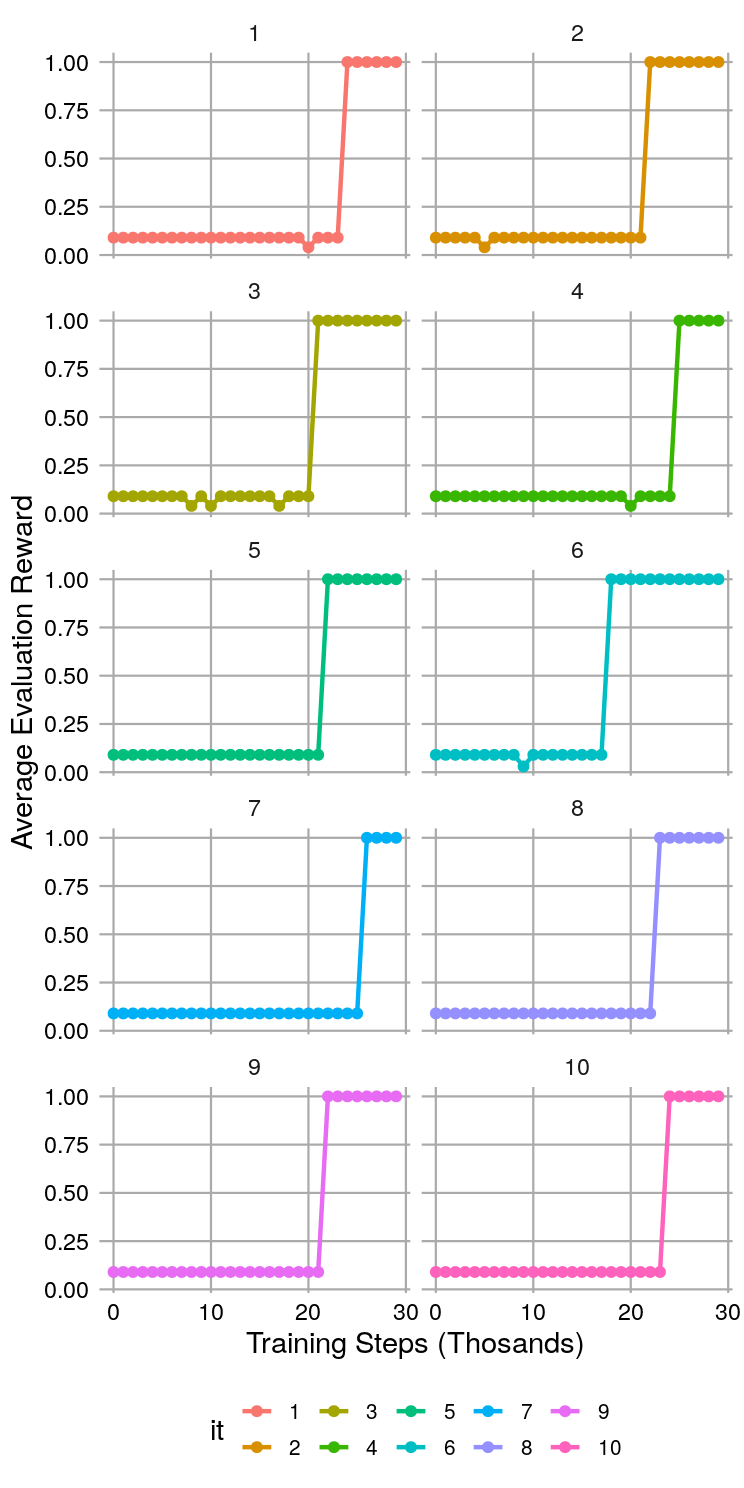
\includegraphics[scale=0.5]{PerDQNCorridor.png}
    }
    \subfloat[BNIG DQN]{
        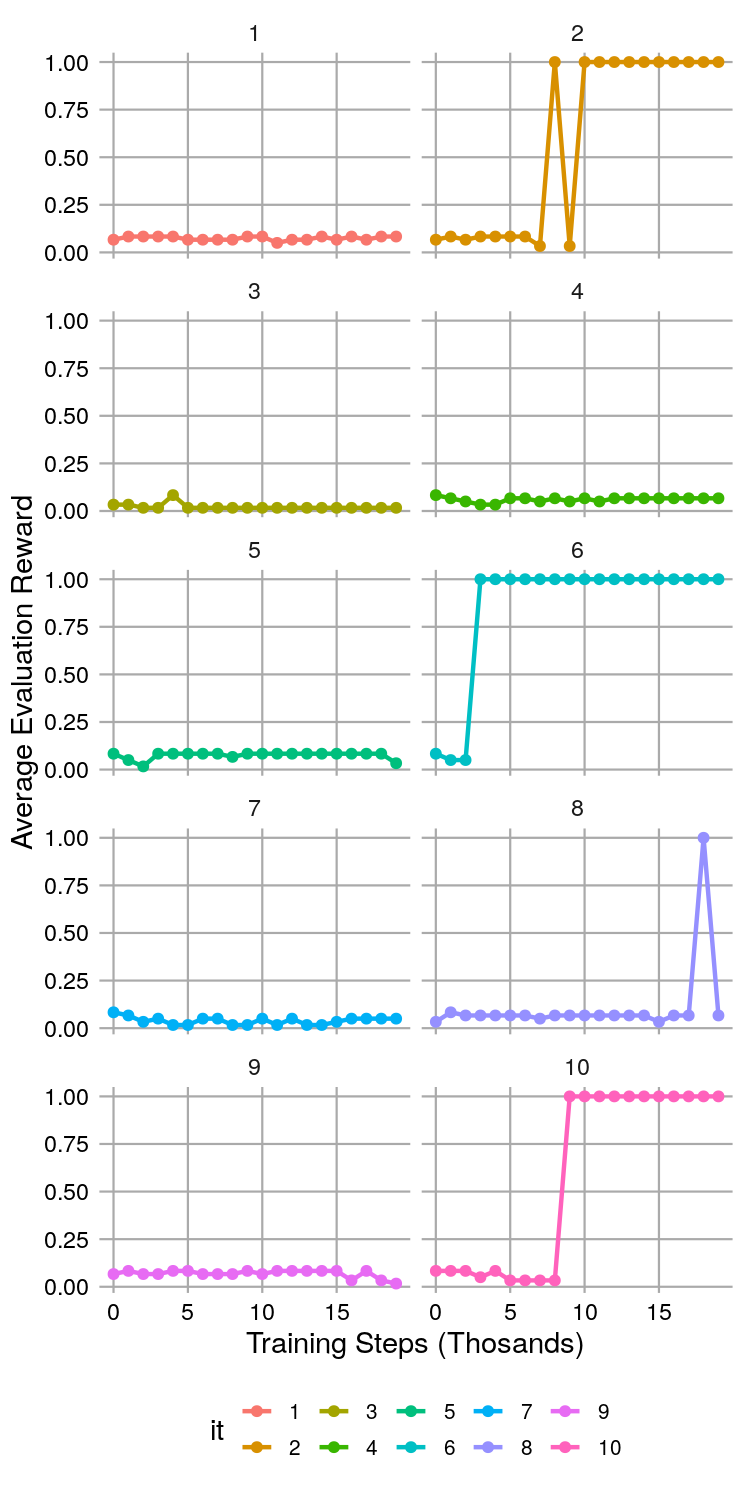
\includegraphics[scale=0.5]{PerBDQNCorridor.png}
    }
    \caption{\textbf{Per Seed DQN and BNIG DQN Performance on Corridor}}
    \label{fig:nn_per_corridor}
\end{figure}

\section{Cartpole}

\begin{figure}[H]
    \centering
    \subfloat[DQN]{
        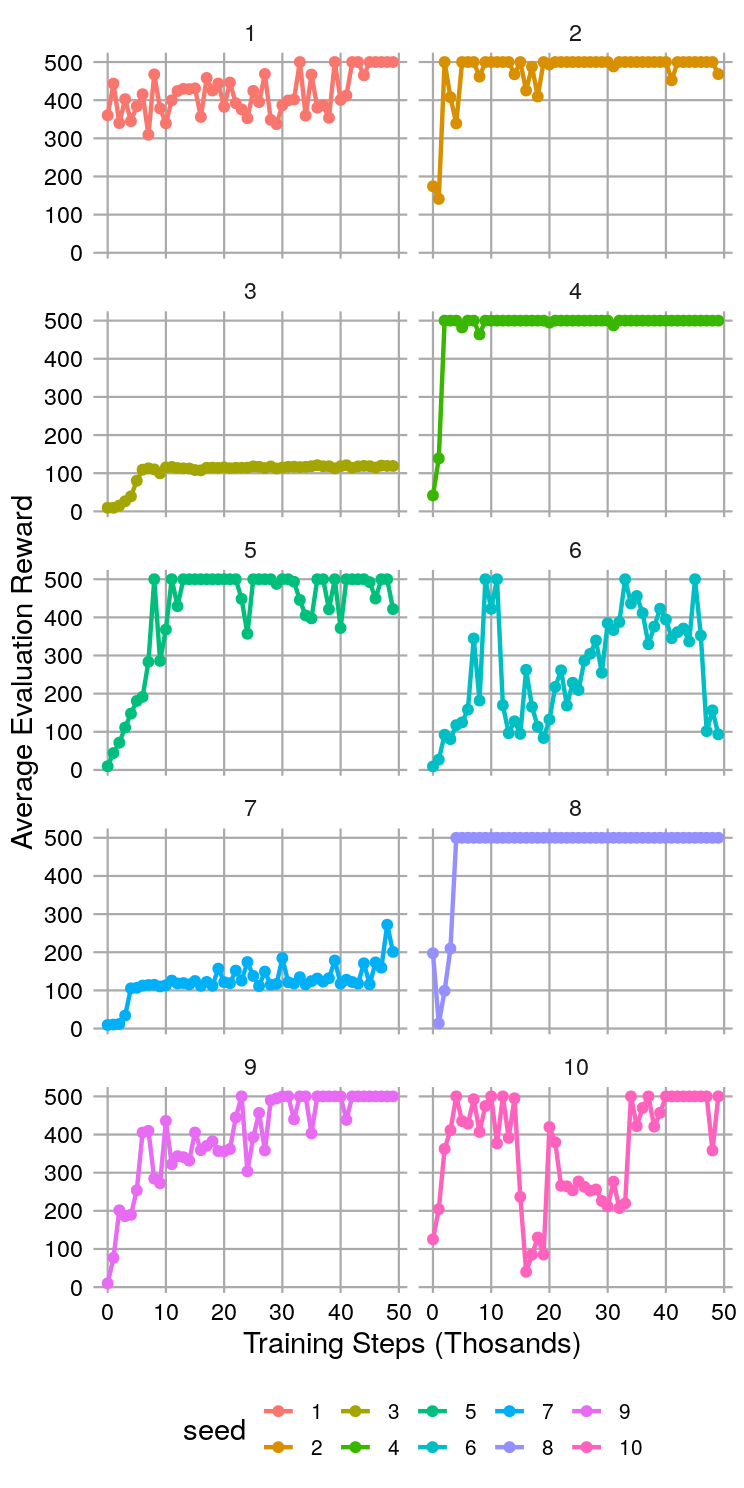
\includegraphics[scale=0.5]{PerDQNCartpole.png}
    }
    \subfloat[BNIG DQN]{
        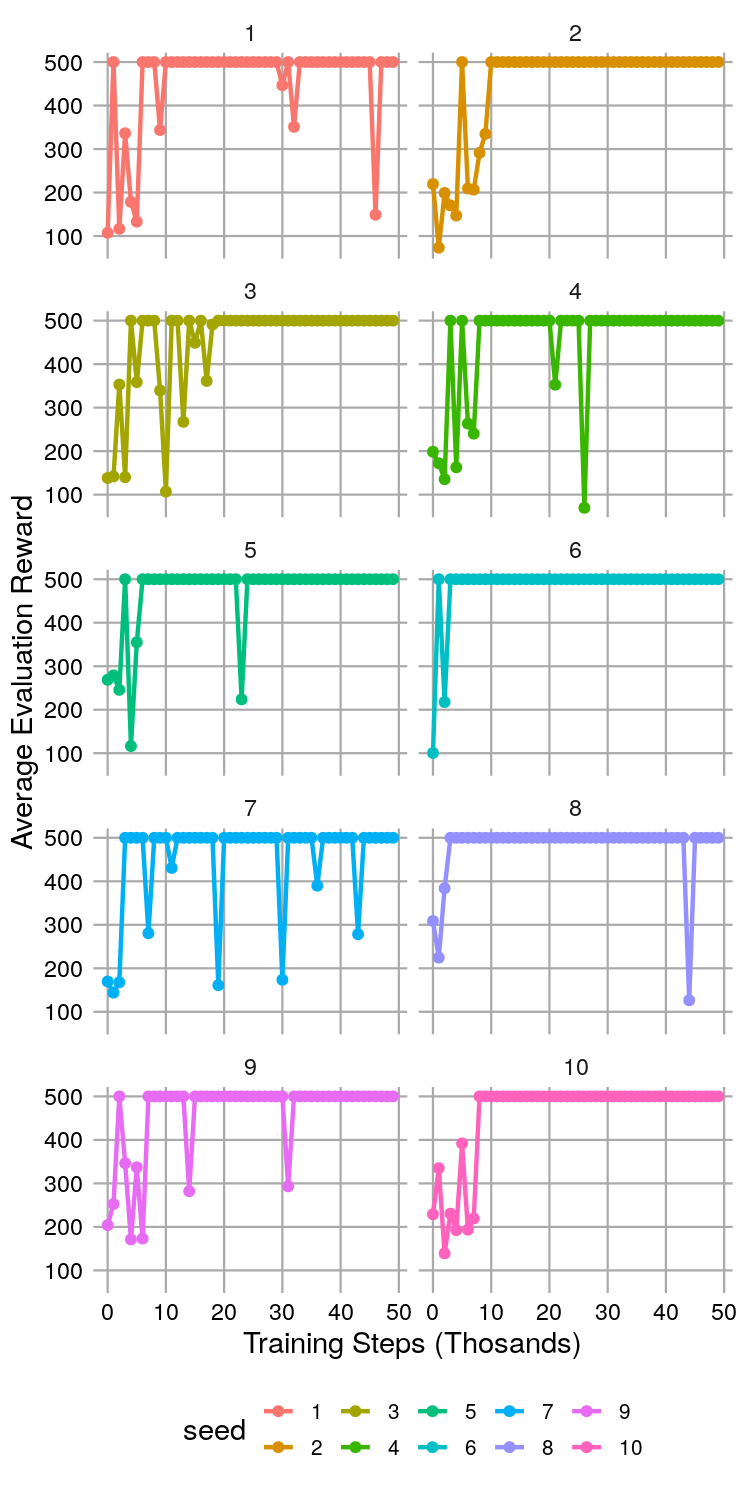
\includegraphics[scale=0.5]{PerBDQNCartpole.png}
    }
    \caption{\textbf{Per Seed DQN and BNIG DQN Performance on Cartpole}: Each color represents a new attempt. Note the unstable performance of DQN when it has found a good policy and that some attempts it never finds an optimal policy.}
    \label{fig:nn_per_cartpole}
\end{figure}

\subsection{Acrobot}

\begin{figure}[H]
    \centering
    \subfloat[DQN]{
        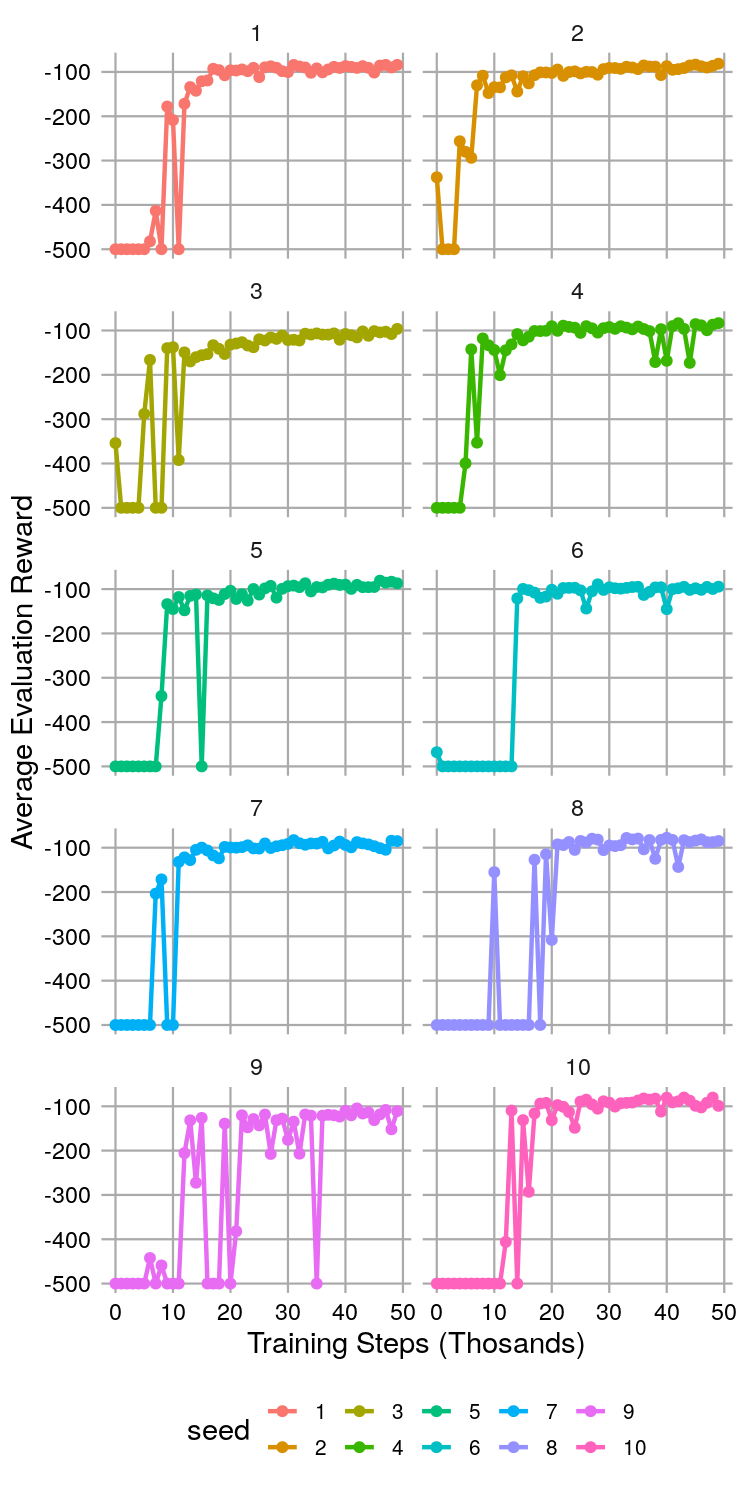
\includegraphics[scale=0.5]{PerDQNAcrobot.png}
    }
    \subfloat[BNIG DQN]{
        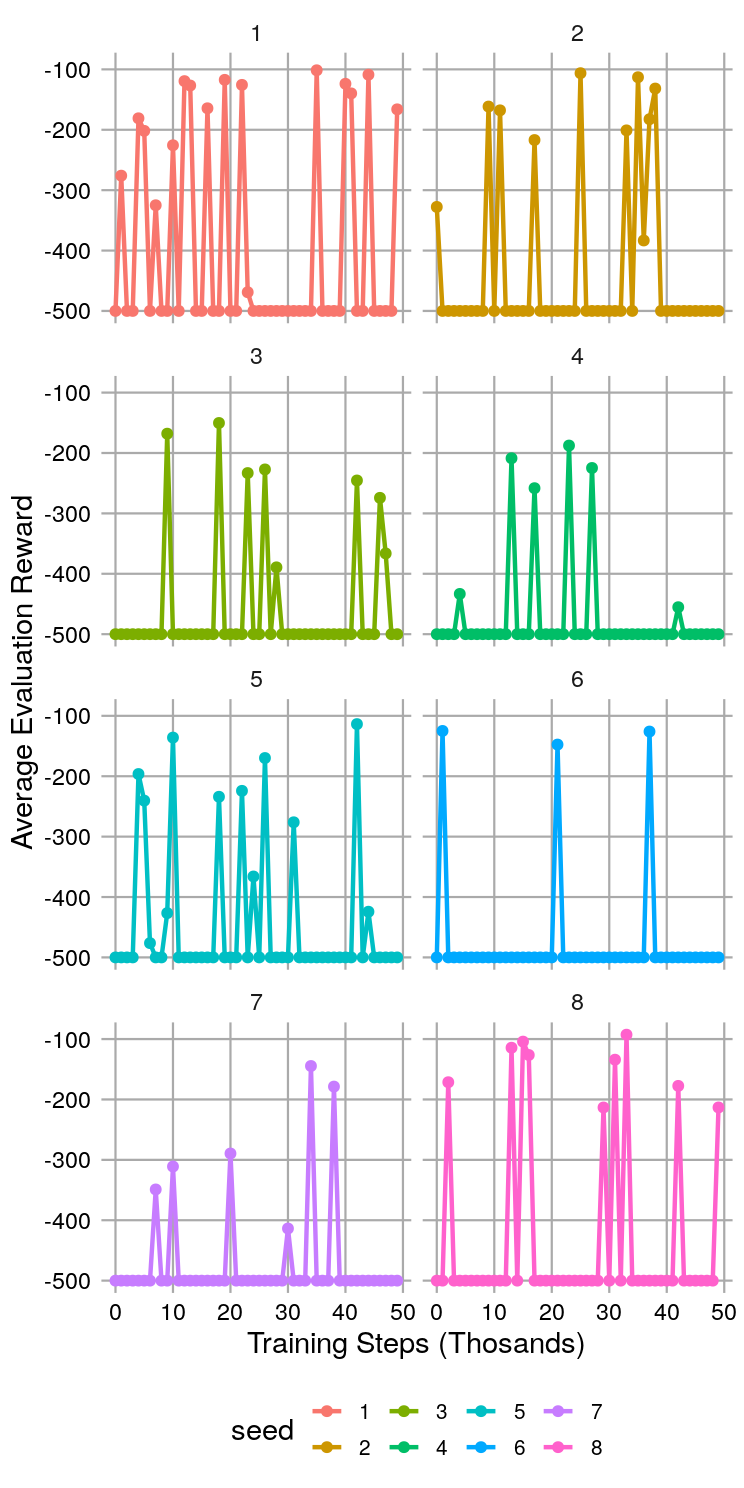
\includegraphics[scale=0.5]{PerBDQNAcrobot.png}
    }
    \caption{\textbf{Per Seed DQN and BNIG DQN Performance on Acrobot}: Each color represents a new attempt. The BNIG DQN occaisonaly finds a good policy, but is not able keep a stable policy.}
    \label{fig:nn_per_acrobot}
\end{figure}
